\documentclass[conference]{IEEEtran}
\usepackage[T1]{fontenc}
\usepackage[utf8]{inputenc}
\usepackage{amsmath,amssymb,booktabs,graphicx,url}
\usepackage[hidelinks]{hyperref}
\usepackage{microtype,tikz}
\usetikzlibrary{arrows.meta,positioning,calc}
\setlength{\emergencystretch}{3em}

\begin{document}

\title{RC-QASyn: Auditable Evidence, Coverage-Aware Construction and Bounded Repair for Synthetic Tabular Data}

\author{\IEEEauthorblockN{Author 1 (to be supplied)}
\IEEEauthorblockA{\textit{Department} \\
\textit{Sardar Vallabhbhai National Institute of Technology}\\
Surat, India \\
email}
\and
\IEEEauthorblockN{Author 2 (to be supplied)}
\IEEEauthorblockA{\textit{Department} \\
\textit{Sardar Vallabhbhai National Institute of Technology}\\
Surat, India \\
email}}

\maketitle

\begin{abstract}
Among 601 historical synthetic tabular candidate occurrences from three imbalanced classification datasets, 75 (12.5\%) violate source-declared structural requirements; page-blocks0 accounts for 64 violations among 200 candidates (32\%). RC-QASyn makes these defects, statistical support and dataset contribution separately auditable through provenance, schema checks, local and global TRAIN evidence, descriptive admission, fixed-budget construction and bounded integer repair. All 54 eligible repairs become structurally compliant; 21 rejected records remain ineligible. At matched budgets, quality-coverage selection raises distinct-feature TRAIN coverage over source order from 0.622 to 0.948 on Abalone19 and from 0.416 to 0.506 on Ecoli4, with zero exact duplicates. Improved geometry does not ensure improved classification: expanding the repaired page-blocks0 pool lowers logistic pure-synthetic F1 from 0.446 to 0.342 (paired conditional 95\% difference interval: $[-0.135,-0.074]$). A separate train-only offline study uses five fresh stratified splits per dataset. Curated augmentation yields mean F1 $0.758\pm0.166$ on Ecoli4 versus $0.848\pm0.119$ for real-only training; gains on page-blocks0 are small and random curation remains competitive. Saved predictions support 2,000-resample paired intervals. An exploratory addendum, declared after the main study, adds six KEEL datasets, re-implemented CLLM-style and discriminator-realism curators and four published oversamplers under the same splits: quality-coverage again covers more TRAIN support than random selection on every new dataset with a usable pool, but shows no consistent F1 or average-precision advantage over random selection or the published methods. These results establish reproducible structural and geometric effects with mixed utility outcomes, without independently establishing complete semantic validity.
\end{abstract}
\begin{IEEEkeywords}
synthetic tabular data; curation; coverage; bounded repair; imbalanced learning
\end{IEEEkeywords}

\section{Introduction}
A generated record can be readable and numerically plausible while omitting its class, violating an integer declaration or duplicating another record. These failures occur in the studied population: 75 of 601 candidates violate authoritative structure, including 64 of 200 page-blocks0 records. These are rates for this historical generation campaign, not estimates for LLM outputs generally. They motivate checking what a record contains before interpreting distributional resemblance or downstream usefulness.

Three questions remain distinct. Does a candidate comply with justified source declarations? How well does it resemble TRAIN observations locally and globally? What does it contribute to a selected dataset and its classifier? A distant observation may be legitimate, a compliant record may be redundant, and a diverse subset may train a worse classifier. RC-QASyn addresses these distinctions with an auditable curation system.

We ask: to what extent do structural filtering, heterogeneous evidence, coverage-aware selection and bounded repair improve measurable synthetic-data characteristics and downstream classification utility compared with simple alternatives? The revision combines a controlled historical study with a separate offline replication. Annotation experiments and validity calibrators are outside the active scope.

The contributions are:
\begin{enumerate}
\item Auditable separation of source-schema compliance, local/global statistical support and dataset contribution, linked to immutable candidate identities.
\item Evidence-aware fixed-budget construction evaluated against random, source-order, farthest-first and coverage-greedy controls, with coverage and redundancy measurements.
\item Source-preserving bounded integer repair, controlled reevaluation and matched-budget measurement of structural, geometric and utility changes.
\item Empirical analysis of agreement and disagreement between geometry and classification, strengthened by paired prediction uncertainty and split-specific offline generation.
\end{enumerate}
These are integration and empirical contributions. Distances, covariance regularization, greedy selection, oversampling and bootstrap methods are established components; no new optimality guarantee is claimed.

\section{Related work}\label{sec:related}
\subsection{Tabular generation}
CTGAN, TabDDPM and GReaT model tabular generation through conditional adversarial, diffusion and language-model approaches \cite{xu2019ctgan,kotelnikov2023tabddpm,borisov2023great}. EPIC adapts LLM prompting specifically to imbalanced-class tabular synthesis \cite{kim2024epic}. These methods change how candidates are produced. RC-QASyn instead curates an existing candidate stream: the historical generator is not retrained here, and the offline experiments do not reproduce its LLM behavior.

\subsection{Curating generated tabular data}
The closest prior work also filters or ranks generated records after generation. CLLM curates LLM-generated rows in low-data regimes using a classifier's learning dynamics, keeping samples with high confidence and low aleatoric uncertainty \cite{seedat2024cllm}. ReFine filters LLM output to suppress redundancy that concentrates in local regions while retaining rare records \cite{jiang2025refine}. Team-then-Trim follows LLM generation with a three-stage plug-in quality-control pipeline \cite{zhang2026t2}. RUBRIC ranks minority candidates from any oversampler by a learned density-ratio realism score combined with a boundary-utility score, then keeps a limited budget \cite{yu2026rubric}. RC-QASyn differs in three respects. Its support evidence is model-free (TRAIN-scaled nearest-neighbour distance and shrinkage Mahalanobis distance) rather than learned. Its admission keeps reject, abstain and review outcomes explicit instead of a single keep/drop decision. It adds source-declared structural checks and bounded repair, which these methods do not address. We do not claim that this design outperforms learned curation; Section~\ref{sec:limitations} records the absence of a direct comparison.

\subsection{Evaluation, coverage and subset selection}
Synthetic-data evaluation can distinguish fidelity, diversity and generalization at sample level \cite{alaa2022faithful}. Density and coverage metrics define support through $k$-nearest-neighbour balls around real observations \cite{naeem2020reliable}; our TRAIN coverage within a fixed radius is closely related, and our duplication rates are narrower diagnostics without probabilistic or privacy interpretation. Greedy coverage and diversity-based subset selection have substantial prior literature \cite{nemhauser1978submodular,sener2018coreset}. Adaptive maximum-coverage sampling has recently been applied to synthetic training data, where a well-chosen subset can outperform the full synthetic set \cite{tavakkol2025less}. We reuse these ideas with traceable admission, class quotas and duplicate suppression. Classical unconstrained greedy guarantees do not automatically extend to the combined lexicographic selector. Quality filtering can also remove modes and reduce diversity in synthetic tabular data \cite{stevenson2026collapse}, which motivates keeping coverage as an explicit objective rather than filtering on fidelity alone.

\subsection{Validation, constraints and repair}
Schema-based data validation is established practice in machine-learning pipelines \cite{breck2019validation}. Constraint-aware models enforce explicit constraints during or immediately after generation \cite{stoian2024realistic}, and recent work discovers inter-column constraints and repairs the records of unchanged generators with a post-processor \cite{zhao2026constraint}. RC-QASyn checks only source-justified declarations and permits a deliberately narrow, integer-only correction with an explicit edit budget, so that repairs remain auditable and never fabricate labels or features.

\subsection{Oversampling and imbalanced learning}
SMOTE interpolates minority observations \cite{chawla2002smote}. Cleaning steps such as Tomek links and edited nearest neighbours remove synthetic or real samples after oversampling \cite{batista2004study}, and SMOTE-IPF applies an ensemble noise filter after SMOTE \cite{saez2015smoteipf}; both are close in spirit to support-based admission. We use established imbalanced-learn implementations, including mixed-type SMOTENC \cite{lemaitre2017imbalanced}. Oversampling is a generation/training baseline, random candidate selection is a curation control, and class weighting changes classifier training. They answer different questions.

\subsection{Calibration and inference}
Calibration concerns agreement between confidence and observed outcomes \cite{guo2017calibration}; candidate percentiles lack that interpretation. Bootstrap inference depends on its resampling design \cite{efron1979bootstrap}, and supplementary Wilson recall intervals address small positive counts \cite{brown2001interval}. Synthetic-data surveys and LLM-judge studies motivate traceability while limiting what recorded critic decisions establish \cite{long2024survey,zheng2023judging}.

\section{Methodology}
Let $T$ denote REAL TRAIN, $E$ REAL TEST and $G=\{(o_i,x_i,y_i)\}$ the candidate stream. Occurrence identity distinguishes physical records with equal payloads, and source files, ordinals, payload hashes, specifications and experiment identities link each selected record to its inputs. A missing class stays missing; generation conditioning never supplies it.

\begin{figure*}[!t]\centering\resizebox{\textwidth}{!}{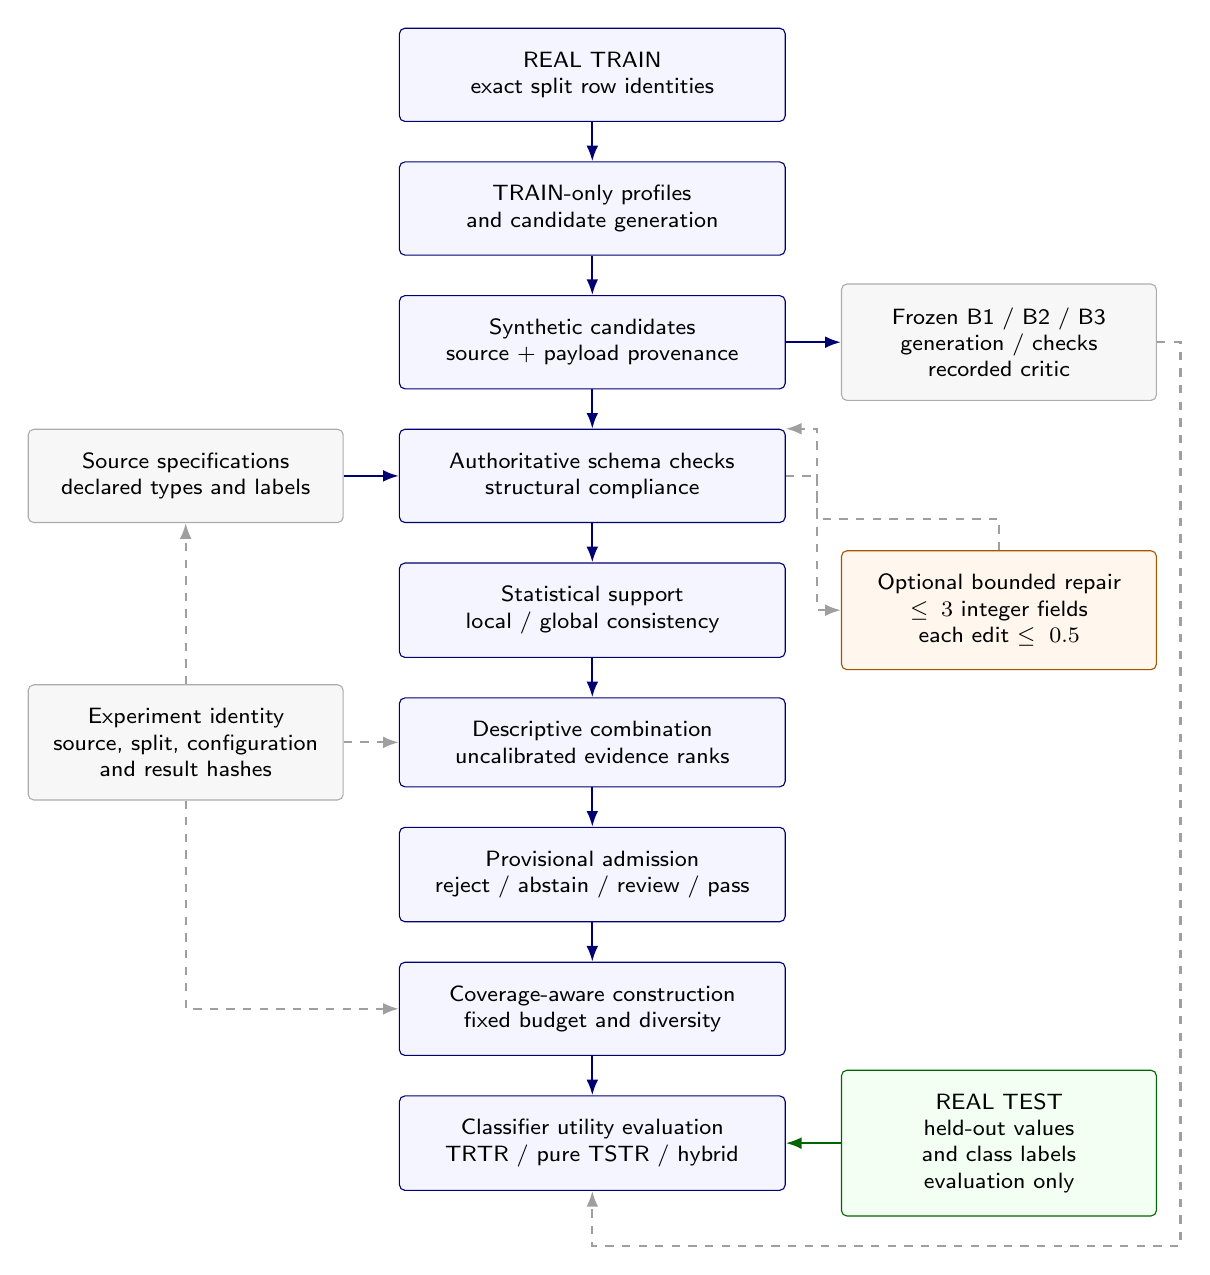
\begin{tikzpicture}[font=\sffamily\footnotesize,
 box/.style={draw=blue!45!black,fill=blue!4,rounded corners=2pt,align=center,text width=43mm,minimum height=10mm,inner sep=3mm},
 side/.style={box,text width=34mm,fill=gray!6,draw=gray!65},
 flow/.style={-{Latex[length=2mm]},thick,draw=blue!45!black},
 audit/.style={flow,dashed,draw=gray!75},node distance=5mm]
\node[box] (train) {REAL TRAIN\\exact split row identities};
\node[box,below=of train] (fit) {TRAIN-only profiles\\and candidate generation};
\node[box,below=of fit] (candidate) {Synthetic candidates\\source + payload provenance};
\node[box,below=of candidate] (schema) {Authoritative schema checks\\structural compliance};
\node[box,below=of schema] (evidence) {Statistical support\\local / global consistency};
\node[box,below=of evidence] (fusion) {Descriptive combination\\uncalibrated evidence ranks};
\node[box,below=of fusion] (admit) {Provisional admission\\reject / abstain / review / pass};
\node[box,below=of admit] (select) {Coverage-aware construction\\fixed budget and diversity};
\node[box,below=of select] (eval) {Classifier utility evaluation\\TRTR / pure TSTR / hybrid};
\node[side,left=7mm of schema] (spec) {Source specifications\\declared types and labels};
\node[side,left=7mm of fusion] (identity) {Experiment identity\\source, split, configuration\\and result hashes};
\node[side,right=7mm of candidate] (controls) {Frozen B1 / B2 / B3\\generation / checks\\recorded critic};
\node[side,right=7mm of evidence,fill=orange!7,draw=orange!65!black] (repair) {Optional bounded repair\\$\le3$ integer fields\\each edit $\le0.5$};
\node[side,right=7mm of eval,fill=green!5,draw=green!40!black] (test) {REAL TEST\\held-out values\\and class labels\\evaluation only};
\foreach \a/\b in {train/fit,fit/candidate,candidate/schema,schema/evidence,evidence/fusion,fusion/admit,admit/select,select/eval}
 \draw[flow] (\a) -- (\b);
\draw[flow] (spec) -- (schema);
\draw[audit] (identity.north) -- (spec.south);
\draw[audit] (identity.east) -- (fusion.west);
\draw[audit] (identity.south) |- (select.west);
\draw[flow] (candidate.east) -- (controls.west);
\draw[audit] (schema.east) -- ++(4mm,0) |- (repair.west);
\draw[audit] (repair.north) -- ++(0,4mm) -| ([xshift=4mm]schema.north east) -- (schema.north east);
\draw[audit] (controls.east) -- ++(3mm,0) |- ([yshift=-7mm]eval.south) -- (eval.south);
\draw[flow,draw=green!40!black] (test.west) -- (eval.east);
\end{tikzpicture}
}
\caption{RC-QASyn architecture. Structure and statistical support are separate; optional repair creates derived versions and repeats checks. B1/B2/B3 remain frozen controls, and REAL TEST enters only evaluation. Dashed arrows denote provenance or optional reevaluation.}\label{fig:architecture}\end{figure*}

\subsection{Structure and statistical evidence}
Specifications declare required features and class, numerical primitives, nominal values, integer fields and permitted fields. Supported violations can reject; observed ranges are not treated as physical bounds. For $p$ features, the TRAIN-scaled mixed distance is
\begin{equation}
d(x,t)=\frac1p\sum_j\delta_j(x_j,t_j),\quad
\delta_j=\begin{cases}\min(|x_j-t_j|/R_j,1),&\text{numeric},R_j>0,\\
\mathbf1[x_j\ne t_j],&\text{nominal or }R_j=0,
\end{cases}
\end{equation}
where $R_j$ is the TRAIN span and class is excluded. Local support $L_k(x)$ averages distances to the nearest $\min(k,|T_s|)$ supported TRAIN observations (ties broken by row identity; primary $k=5$). Global consistency scales numerical features by TRAIN median/IQR (falling back to span, then one), one-hot encodes TRAIN categories and, for encoded dimension $D$, covariance $S$ and mean $\mu$, uses
\begin{equation}
\Sigma=(1-\alpha)S+\alpha\operatorname{diag}(S)+\lambda I,\qquad
Q(x)=\sqrt{\max(0,(z-\mu)^\top\Sigma^{-1}(z-\mu))/D},
\end{equation}
with primary $\alpha=.10$, $\lambda=10^{-8}$. Unsupported evidence and unseen categories stay explicit.

\subsection{Descriptive combination and admission}
For the reference set $A_f$ of candidate scores in a dataset and evidence family,
\begin{equation}
u_f(s)=\bigl(\#\{a<s\}+\tfrac12\#\{a=s\}\bigr)/|A_f|,
\end{equation}
where larger ranks mean weaker support. Combined concern $\max(u_L,u_Q)$ requires both components and is an uncalibrated index, not a validity probability; no independence assumption or learned weight is used. Admission rejects authoritative defects, abstains when required evidence is missing, requests review for partial structure or concern of at least $q=.90$, and otherwise provisionally passes. Structure, local and global policies form ablations, and $q=.80,.95$ are historical sensitivities. Track A keeps historical models and ranks, including for derived queries; Track B recomputes them for each new TRAIN-fitted pool.

\subsection{Coverage-aware construction}
Let $\mathcal R$ be the distinct TRAIN feature/class regions and $h_t(S)=\mathbf1[\min_{s\in S}d(s,t)\le .05]$. Uniform coverage averages $h_t$ over regions, balanced coverage weights each class-$y$ region by $1/(K n_y)$, and distinct-feature TRAIN coverage is reported separately. At budget $b$, source order takes the earliest occurrences, farthest-first maximizes minimum separation and coverage-greedy maximizes uniform marginal coverage. Quality-coverage forbids repeated feature payloads, first fills a feasible minority quota $\lfloor .5b\rfloor$, and then ranks lexicographically by balanced marginal coverage, fewer neighbours within $.01$, greater separation, lower concern and source order. Exact redundancy is $1-u/n$ for $u$ unique payloads among $n$ selections; near redundancy is the fraction of selections with another within $.01$.

\subsection{Bounded structural repair}
Only fractional finite values in source-declared integer fields can change. Decimal half-to-even rounding must satisfy
\begin{equation}
|J|\le3,\quad |x'_j-x_j|\le .5\ (j\in J),\qquad x'_j=x_j\ (j\notin J).
\end{equation}
Missing targets or features, category substitution and imputation are excluded, and a record needing more than three edits is refused. Derived identities bind parent, policy, specification and payload; originals stay immutable, frozen evidence and admission rescore repairs, and parent exclusivity prevents double counting. Expanded-pool comparisons therefore measure repair plus reselection, not the isolated effect of one edit.

\section{Experimental design}
The protocol was committed before any new score was computed (\texttt{91619f1}) on frozen main \texttt{244a9bf}, and settings stay fixed after scoring. The research questions cover structural frequency (RQ1), evidence complementarity (RQ2), coverage and redundancy (RQ3), repair (RQ4), utility (RQ5) and stability and uncertainty (RQ6).
\begin{table}[!t]
\centering
\caption{Frozen task datasets and literal positive counts.}\label{tab:datasets}
\footnotesize\setlength{\tabcolsep}{3pt}
\begin{tabular}{lrrrrrr}
\toprule
Dataset & Rows & TRAIN & TEST & TRAIN+ & TEST+ & Candidates \\
\midrule
Abalone19 & 4174 & 3340 & 834 & 26 & 6 & 200 \\
Ecoli4 & 336 & 269 & 67 & 16 & 4 & 201 \\
page-blocks0 & 5472 & 4377 & 1095 & 447 & 112 & 200 \\
\bottomrule
\end{tabular}
\end{table}


\begin{figure}[!t]\centering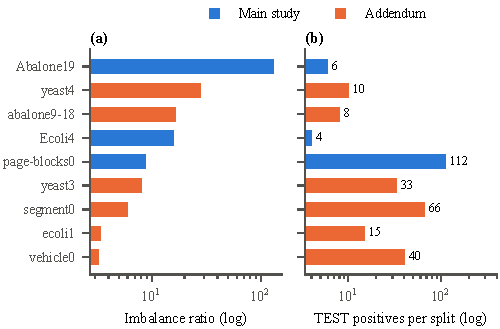
\includegraphics[width=\linewidth]{figures/datasets.pdf}
\caption{Datasets of the main study and the exploratory addendum (Section~\ref{sec:addendum}). (a) Imbalance ratio. (b) TEST positives per fresh split, which bound inference on the smallest datasets.}\label{fig:datasets}\end{figure}

\textit{Track A (historical fixed split).} Datasets, original TRAIN/TEST identities and the 601 candidates are unchanged; candidates depended on original TRAIN and are never reassigned, the previously evaluated TEST set is reused descriptively, and exact TRAIN/TEST feature overlap is recorded. Budgets of 56, 70 and 49 for Abalone19, Ecoli4 and page-blocks0 are inherited. Raw-labeled random keeps evaluable integer defects but excludes absent labels and unsupported features, schema random requires full compliance, and admitted random draws from the combined-admitted pool shared by the four deterministic selectors; random controls use seeds $13,29,43,61,79$. Admission ablations apply the same quality-coverage selector after structure-only, local, global or combined eligibility, so pool size is part of the intervention. All 138 historical utility comparisons are replayed from saved predictions; B1/B2/B3 stay frozen and are intersected with structural completeness. The archived raw scorer could read a missing class as the string \texttt{nan}, so those scores are not used as complete binary-record comparisons. External comparators append exactly $b$ minority rows with ROS or SMOTE (SMOTENC for categorical Abalone19), with TRAIN-fitted standardization and unrounded page-blocks0 integers, and balanced logistic loss is a non-generative comparator. These are training alternatives, not same-pool curation; mixed-class historical subsets may add fewer than $b$ minority rows in hybrid regimes.

\textit{Track B (fresh offline splits).} Five deterministic stratified 80/20 splits per dataset use the same seeds, and every split refits preprocessing, generation, evidence and geometry on its own TRAIN. Pools hold $4b$ minority records from SMOTENC (Abalone19), SMOTE (Ecoli4) or ROS (integer-declared page-blocks0, which adds no new support), with $k=\min(5,n_+-1)$. Six curators (schema random, admitted random, source order, farthest-first, coverage-greedy, quality-coverage) are compared with real-only, class-weighted and ROS/SMOTE training. Minority-only pools allow hybrid augmentation but not pure TSTR. This tests offline curation, not LLM candidate quality, and because holdouts overlap, across-split SD describes variability, not an independent-sample standard error.

\textit{Classifiers, metrics and uncertainty.} Logistic regression (liblinear, at most 300 iterations) and random forest (50 trees) use seed 42, with imputation, scaling and encoding fitted only on the training population. TRTR trains on real TRAIN, pure TSTR on synthetic rows and hybrid on real TRAIN plus synthetic positives. We report $F_1=2TP/(2TP+FP+FN)$, balanced accuracy, MCC, AP (the step integral $\sum_k(R_k-R_{k-1})P_k$, not trapezoidal area) and AUROC; point MCC uses the frozen zero convention for degenerate margins, and undefined cases are counted explicitly. Historical intervals use 2,000 stratified paired resamples of saved predictions (seed 20261025, 95\% percentile bounds), resampling positive and negative indices within strata identically across paired methods. Primary pairs compare original quality-coverage with schema and admitted random (seed 13), hybrid quality-coverage with TRTR, and repaired with original quality-coverage. Intervals condition on fitted models and observed TEST, excluding generation and refitting uncertainty. No multiplicity-adjusted significance claim is made.

\section{Results}
\begin{figure*}[!t]\centering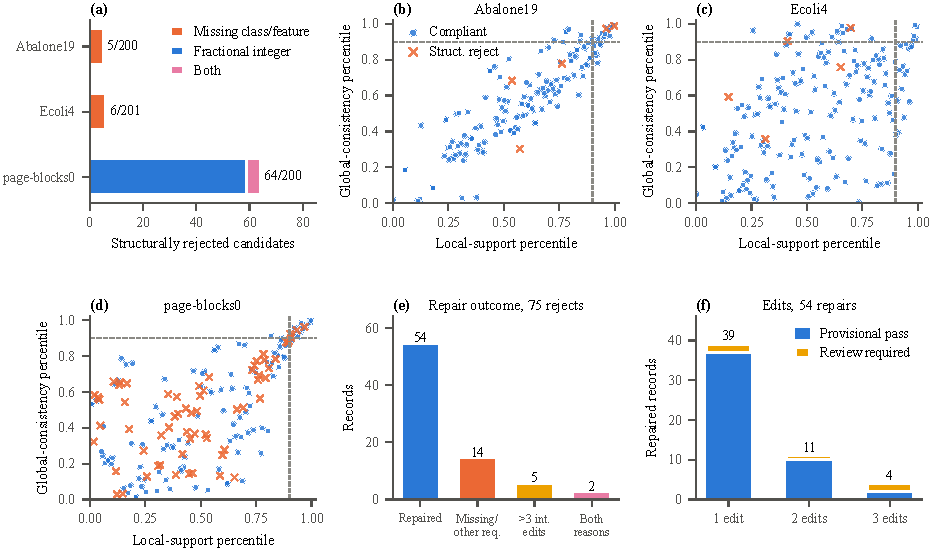
\includegraphics[width=\textwidth]{figures/audit.pdf}
\caption{Historical candidate audit. (a) Structural rejects by violation type. (b--d) Local-support and global-consistency percentiles of every candidate with available evidence; dashed lines mark the review cutoff $q=.90$, crosses mark structural rejects. (e) Repair outcome for the 75 rejects. (f) Integer edits per repaired record and admission after rescoring.}\label{fig:audit}\end{figure*}

\subsection{RQ1--RQ2: structure and complementary support}
There are 75 structural rejects (12.48\%): five of 200 Abalone19, six of 201 Ecoli4 and 64 of 200 page-blocks0 candidates (Fig.~\ref{fig:audit}a). Fifteen lack class, one lacks features and 64 have fractional-integer fields; 26 violate multiple fields, and no unsupported nominal value or invalid numerical primitive appears. Local and global evidence are related but flag different records (Fig.~\ref{fig:audit}b--d): Spearman correlations are $.908$, $.488$ and $.621$ for Abalone19, Ecoli4 and page-blocks0, with 14, 30 and two tail disagreements. Combined admission yields 170, 162 and 119 provisional passes, against 195, 195 and 136 with structure only. This shows distinct statistical information, not semantic-error detection performance.

\subsection{RQ3: matched-budget ablations}
\begin{table*}[!t]
\centering
\caption{Consolidated historical ablations. Q denotes unchanged quality-coverage selection. Random rows average five seeds; complete per-seed data accompany the paper. F1 is logistic pure TSTR; -- means unavailable.}\label{tab:ablations}
\footnotesize\setlength{\tabcolsep}{6pt}
\begin{tabular}{lrrrrrrr}
\toprule
Dataset & Method & Pool & $n$ & Coverage & Exact & Near & F1 \\
\midrule
Abalone19 & Raw labeled random & 195 & 56 & 0.799 & 0.171 & 0.443 & 0.029 \\
 & Schema random & 195 & 56 & 0.799 & 0.171 & 0.443 & 0.029 \\
 & Admitted random & 170 & 56 & 0.833 & 0.236 & 0.493 & 0.022 \\
 & Structure + Q selection & 195 & 56 & 0.951 & 0.000 & 0.000 & 0.030 \\
 & Structure/local + Q & 177 & 56 & 0.950 & 0.000 & 0.000 & 0.031 \\
 & Structure/global + Q & 177 & 56 & 0.948 & 0.000 & 0.000 & 0.031 \\
 & Structure/local/global + Q & 170 & 56 & 0.948 & 0.000 & 0.000 & 0.031 \\
 & Admitted source order & 170 & 56 & 0.622 & 0.357 & 0.625 & -- \\
 & Admitted farthest first & 170 & 56 & 0.940 & 0.000 & 0.000 & 0.035 \\
 & Admitted coverage greedy & 170 & 56 & 0.948 & 0.107 & 0.268 & 0.030 \\
 & Repair pool + Q & 170 & 56 & 0.948 & 0.000 & 0.000 & 0.031 \\
Ecoli4 & Raw labeled random & 195 & 70 & 0.422 & 0.097 & 0.180 & 0.253 \\
 & Schema random & 195 & 70 & 0.422 & 0.097 & 0.180 & 0.253 \\
 & Admitted random & 162 & 70 & 0.439 & 0.117 & 0.197 & 0.217 \\
 & Structure + Q selection & 195 & 70 & 0.509 & 0.000 & 0.000 & 0.216 \\
 & Structure/local + Q & 175 & 70 & 0.509 & 0.000 & 0.000 & 0.195 \\
 & Structure/global + Q & 177 & 70 & 0.506 & 0.000 & 0.000 & 0.229 \\
 & Structure/local/global + Q & 162 & 70 & 0.506 & 0.000 & 0.000 & 0.205 \\
 & Admitted source order & 162 & 70 & 0.416 & 0.200 & 0.386 & -- \\
 & Admitted farthest first & 162 & 70 & 0.468 & 0.000 & 0.000 & 0.200 \\
 & Admitted coverage greedy & 162 & 70 & 0.506 & 0.114 & 0.243 & 0.108 \\
 & Repair pool + Q & 162 & 70 & 0.506 & 0.000 & 0.000 & 0.205 \\
page-blocks0 & Raw labeled random & 195 & 49 & 0.905 & 0.061 & 0.559 & 0.390 \\
 & Schema random & 136 & 49 & 0.889 & 0.069 & 0.559 & 0.477 \\
 & Admitted random & 119 & 49 & 0.914 & 0.082 & 0.702 & 0.535 \\
 & Structure + Q selection & 136 & 49 & 0.934 & 0.000 & 0.286 & 0.202 \\
 & Structure/local + Q & 120 & 49 & 0.932 & 0.000 & 0.327 & 0.446 \\
 & Structure/global + Q & 120 & 49 & 0.934 & 0.000 & 0.327 & 0.448 \\
 & Structure/local/global + Q & 119 & 49 & 0.932 & 0.000 & 0.327 & 0.446 \\
 & Admitted source order & 119 & 49 & 0.914 & 0.265 & 0.592 & -- \\
 & Admitted farthest first & 119 & 49 & 0.932 & 0.000 & 0.000 & 0.550 \\
 & Admitted coverage greedy & 119 & 49 & 0.932 & 0.163 & 0.449 & 0.627 \\
 & Repair pool + Q & 168 & 49 & 0.937 & 0.000 & 0.102 & 0.342 \\
\bottomrule
\end{tabular}
\end{table*}

\begin{figure*}[!t]\centering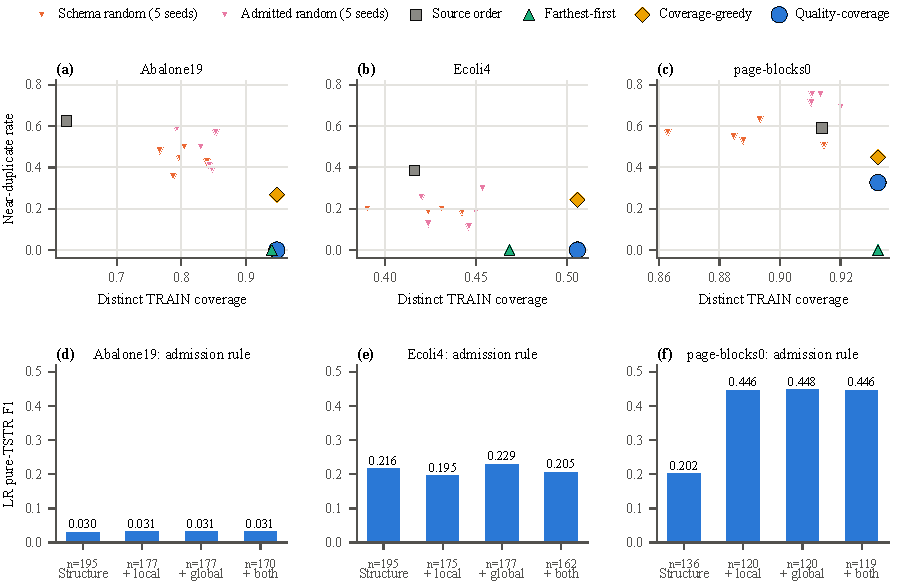
\includegraphics[width=\textwidth]{figures/construction.pdf}
\caption{Historical matched-budget construction. (a--c) Distinct-feature TRAIN coverage against near-duplicate rate; random controls show all five seeds, and deterministic selectors share the admitted pool (on Abalone19, farthest-first and quality-coverage nearly coincide). (d--f) Logistic pure-TSTR F1 after quality-coverage selection under each admission rule; $n$ is the eligible pool.}\label{fig:construction}\end{figure*}
Every construction reaches its budget (Table~\ref{tab:ablations}, Fig.~\ref{fig:construction}). Quality-coverage raises distinct-feature TRAIN coverage over source order from $.6225$ to $.9479$ on Abalone19 and from $.4164$ to $.5056$ on Ecoli4, with zero exact and near redundancy. Farthest-first also removes redundancy but covers less of Ecoli4 ($.4684$); coverage-greedy matches $.5056$ with exact duplication $.1143$. Eligibility, quotas and coverage act together, so this is not the isolated effect of an evidence score. Additional evidence also changes outcomes non-monotonically: structure-only admission slightly exceeds full-admission coverage on Abalone19 ($.951$ versus $.948$) and Ecoli4 ($.509$ versus $.506$), whereas on page-blocks0 full admission raises logistic pure-TSTR F1 from $.202$ to $.446$.

\subsection{RQ4: bounded repair}
All 54 eligible repairs become compliant; 21 rejects are ineligible (Fig.~\ref{fig:audit}e), including five page-blocks0 records that also lack class and five that need more than three edits. Repairs edit 73 fields: 39 records need one edit, eleven two and four three, with absolute changes of $.1$--$.5$ (mean $.3119$). Under unchanged admission, 49 repaired versions provisionally pass and five need review, so the page-blocks0 admitted pool grows from 119 to 168. At budget 49, quality-coverage selects 16 repaired records: coverage rises from $.9324$ to $.9370$ and near duplication falls from $.3265$ to $.1020$. Source-order coverage declines slightly, so expanded pools have method-dependent effects.

\subsection{RQ5: utility and external comparators}
All 138 historical utility rows reproduce within $10^{-12}$. The expanded study has 894 utility rows, 678 successful and 216 explicitly unavailable, with no execution failures or budget shortfalls.
\begin{table*}[!t]
\centering
\caption{Historical external training baselines. ROS and SMOTE/NC append b minority rows. LR: logistic regression; RF: random forest. These differ from candidate curation.}\label{tab:external}
\footnotesize\setlength{\tabcolsep}{6pt}
\begin{tabular}{lrrrrrr}
\toprule
Dataset / method & Model & $+n$ & F1 & AP & BA & MCC \\
\midrule
Abalone19 / Real & LR & 0 & 0.000 & 0.026 & 0.500 & 0.000 \\
Abalone19 / Real & RF & 0 & 0.000 & 0.023 & 0.500 & 0.000 \\
Abalone19 / Weighted LR & LR & 0 & 0.054 & 0.038 & 0.873 & 0.144 \\
Abalone19 / ROS+b & LR & 56 & 0.000 & 0.031 & 0.500 & 0.000 \\
Abalone19 / ROS+b & RF & 56 & 0.000 & 0.031 & 0.500 & 0.000 \\
Abalone19 / SMOTENC+b & LR & 56 & 0.000 & 0.014 & 0.499 & -0.003 \\
Abalone19 / SMOTENC+b & RF & 56 & 0.000 & 0.020 & 0.499 & -0.003 \\
Ecoli4 / Real & LR & 0 & 1.000 & 1.000 & 1.000 & 1.000 \\
Ecoli4 / Real & RF & 0 & 0.667 & 1.000 & 0.750 & 0.696 \\
Ecoli4 / Weighted LR & LR & 0 & 0.800 & 1.000 & 0.984 & 0.803 \\
Ecoli4 / ROS+b & LR & 70 & 1.000 & 1.000 & 1.000 & 1.000 \\
Ecoli4 / ROS+b & RF & 70 & 0.857 & 1.000 & 0.875 & 0.859 \\
Ecoli4 / SMOTE+b & LR & 70 & 1.000 & 1.000 & 1.000 & 1.000 \\
Ecoli4 / SMOTE+b & RF & 70 & 0.857 & 1.000 & 0.875 & 0.859 \\
page-blocks0 / Real & LR & 0 & 0.715 & 0.746 & 0.802 & 0.699 \\
page-blocks0 / Real & RF & 0 & 0.869 & 0.921 & 0.911 & 0.856 \\
page-blocks0 / Weighted LR & LR & 0 & 0.721 & 0.768 & 0.903 & 0.696 \\
page-blocks0 / ROS+b & LR & 49 & 0.728 & 0.746 & 0.811 & 0.712 \\
page-blocks0 / ROS+b & RF & 49 & 0.864 & 0.920 & 0.906 & 0.851 \\
page-blocks0 / SMOTE+b & LR & 49 & 0.728 & 0.758 & 0.811 & 0.712 \\
page-blocks0 / SMOTE+b & RF & 49 & 0.869 & 0.916 & 0.911 & 0.856 \\
\bottomrule
\end{tabular}
\end{table*}

The external baselines (Table~\ref{tab:external}) are training alternatives, not matched curation. Standard SMOTE output for page-blocks0 is not integer-coerced, so 46 of 49 generated rows fail the integer contract while remaining evaluable numerical augmentation.

Geometry and utility can disagree. For page-blocks0 logistic pure TSTR, repair-pool expansion lowers F1 from $.4464$ to $.3421$, while AP moves from $.5552$ to $.5716$ and hybrid F1 stays $.7150$, despite the coverage and redundancy gains of RQ4.

\subsection{RQ6: conditional uncertainty and fresh-split stability}
\begin{figure*}[!t]\centering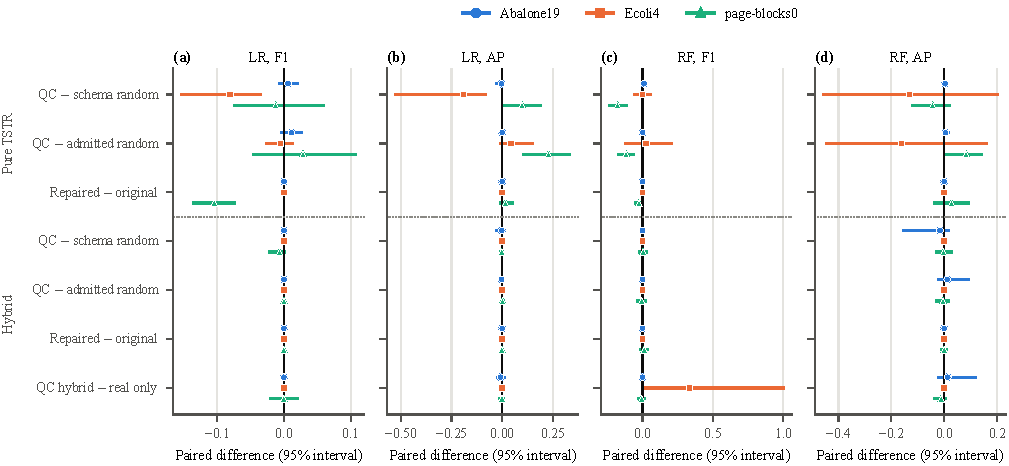
\includegraphics[width=\textwidth]{figures/uncertainty.pdf}
\caption{Conditional paired 95\% intervals for the primary historical pairs (2,000 stratified resamples of saved predictions); markers are observed differences. Intervals condition on the fitted models and the reused historical TEST set; endpoint intervals are in Appendix Table~\ref{tab:bootstrap}.}\label{fig:uncertainty}\end{figure*}
Saved predictions give 216 endpoint and 168 paired-difference intervals (Fig.~\ref{fig:uncertainty}). The page-blocks0 logistic repair-minus-original F1 difference is about $-.1043$ (interval $[-.1350,-.0739]$) and the AP difference $.0165$ ($[-.0071,.0493]$): F1 decreases consistently under this design, while the AP direction is less stable. Small positive counts limit the rest. Ecoli4 logistic TRTR predicts its four positive and 63 negative TEST records perfectly, giving F1 interval $[1,1]$ but a Wilson positive-recall interval of about $[.510,1]$, and Abalone19 has six TEST positives; resampling adds no independent positive observations.

\begin{figure*}[!t]\centering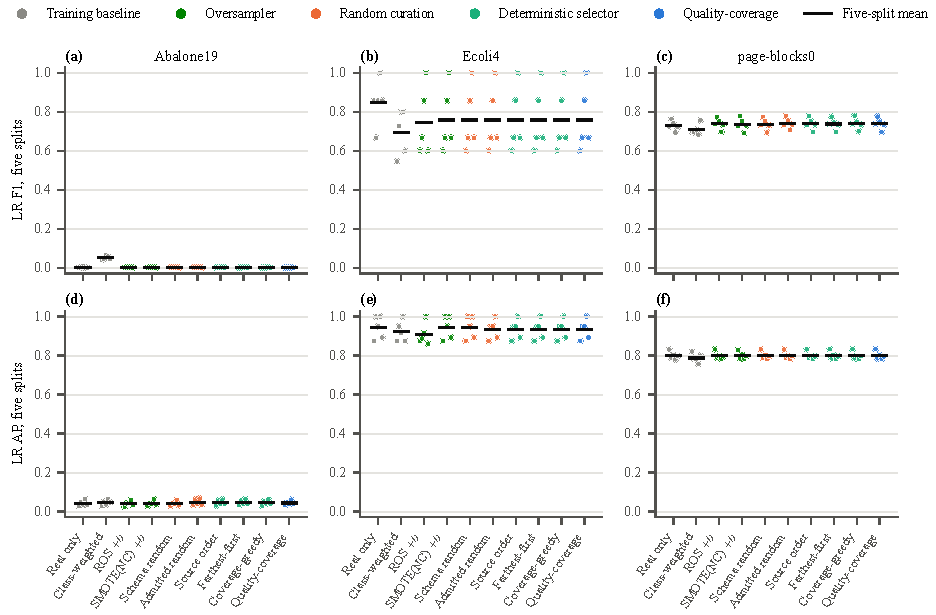
\includegraphics[width=\textwidth]{figures/fresh-splits.pdf}
\caption{Offline replication on five fresh stratified splits: logistic F1 (a--c) and AP (d--f) per split with five-split means. Curators use the hybrid regime; real-only and class-weighted training use TRTR; the page-blocks0 pool generator is ROS. Summary statistics are in Appendix Table~\ref{tab:repeated}.}\label{fig:fresh}\end{figure*}
All 15 split-specific runs complete (Fig.~\ref{fig:fresh}). Ecoli4 logistic F1 is $.8476\pm.1186$ for real-only training and $.7581\pm.1659$ for quality-curated augmentation, the same mean as admitted random. Abalone19 F1 stays zero under real-only training and every augmentation method, while balanced logistic loss reaches $.0506\pm.0095$. On page-blocks0, real-only F1 is $.7284\pm.0256$, quality-curated augmentation $.7383\pm.0283$ and admitted random $.7409\pm.0270$. Augmentation brings no uniform benefit and does not beat simple curation.

\section{Discussion}
The strongest empirical contribution is a measurable separation of compliance, support, geometry and utility. Structural defects are frequent enough in this historical stream to motivate explicit checks, and narrow repair corrects an eligible subset without fabricating labels. Coverage-oriented construction reduces redundancy, but its classifier consequences are mixed, so geometric evidence should accompany direct task evaluation. Admission ablations measure the effect of changing candidate availability under fixed downstream rules, not a score's isolated utility effect, and repair changes both pool and selection, so its utility decrease cannot be assigned to rounding one field. Source order can exclude the minority entirely, which makes unavailable TSTR a meaningful result rather than a reason to add ineligible data. Simple alternatives are informative: farthest-first eliminates duplicates, random selection stays competitive offline, and balanced logistic loss gives nonzero Abalone19 F1 where fixed-budget augmentation does not. The contribution is auditable curation with explicit tradeoffs, not universally better classifier training.

\section{Limitations}\label{sec:limitations}
\textit{Data and splits.} The historical study uses three datasets, a previously evaluated TEST set with recorded TRAIN/TEST overlap, and a pool generated from full original TRAIN, which prevents independent split claims. The fresh study rebuilds every fitted object, but its holdouts overlap, its generators differ from the LLM stream, ROS adds no new support and minority-only pools preclude pure TSTR. Offline findings, including the addendum, do not replicate LLM generation.

\textit{Inference.} Ecoli4 and Abalone19 have four and six historical TEST positives, and abalone9-18 and yeast4 have eight and ten per split. Stratified intervals condition on observed records and fixed models, quantify neither generation nor refitting uncertainty, and cannot discover unseen positive modes; excluding undefined MCC margins can change the conditional target. All comparisons are exploratory, with no multiplicity-adjusted significance or state-of-the-art claim.

\textit{Validity.} Source declarations are a limited contract: physical constraints, target meaning and cross-field semantics stay unresolved where sources cannot justify them. Without a human annotation experiment, complete semantic validity is not independently established; LLM-proposed labels from an earlier phase for the 120-record audit sample (27 invalid, all structural; 93 indeterminate; none confirmed valid) are not ground truth and are unused. Evidence is uncalibrated, provisional admission is a selection policy rather than verified validity, distances depend on scaling and covariance assumptions, and coverage establishes neither predictive accuracy nor privacy.

\textit{Baselines and addendum.} The utility evidence does not favour the proposed selector. Equal-budget B1 and B3 comparisons are unreported (B3 would need new judge calls), and the learned curators re-implement principles of CLLM and RUBRIC's realism component without CLLM's LLM generation or RUBRIC's boundary-utility term. The addendum was designed after the main results and review were known, so it tests declared questions rather than replicating independently. Several datasets share KEEL sources (yeast3/yeast4, Ecoli4/ecoli1, Abalone19/abalone9-18), so dataset-level tests overstate the effective sample. Re-scoring the canonical comparators on another platform changes some metrics by up to $.0097$, and the published AUROC comparison uses a different protocol. Structural checks and repair are exercised mainly on the historical LLM stream; on vehicle0, the only fresh pool with defects, the three-edit bound recovers six of 1{,}400 candidates, so the repair policy does not suit interpolation output.

\textit{Future work.} Open directions are independent datasets with more minority TEST records beyond the KEEL derivatives used here, a second LLM generation campaign under fresh splits, structural rules and repair bounds designed for interpolation output, equal-budget B1 and B3 comparisons with full learned-curation implementations, and blinded human validity labels for the audit sample.

\section{Conclusion}
RC-QASyn makes provenance, structural compliance, statistical support, fixed-budget construction and bounded repair inspectable within the existing six-phase system. The historical audit identifies 75 structural rejects, repairs all 54 eligible records and measures the resulting changes in coverage and redundancy. Paired uncertainty and fresh train-only experiments strengthen the evidence while revealing limited and sometimes negative utility effects, and an exploratory addendum on nine datasets reproduces the geometric gain without a utility advantage over random selection, re-implemented learned curators or published oversamplers. The contribution is an empirically bounded, reproducible account of curation tradeoffs.


\bibliographystyle{IEEEtran}
\bibliography{references}

\appendices
\section{Class denominators and confusion counts}
\begin{table*}[!t]
\centering
\caption{Historical primary predictions: class denominators and confusion counts. Q and Q repair use pure TSTR; Real uses TRTR.}\label{tab:confusions}
\footnotesize\setlength{\tabcolsep}{6pt}
\begin{tabular}{lrrrrrrr}
\toprule
Dataset / method & Model & $n_+$ & $n_-$ & TP & FP & TN & FN \\
\midrule
Abalone19 / Real & LR & 6 & 828 & 0 & 0 & 828 & 6 \\
Abalone19 / Real & RF & 6 & 828 & 0 & 0 & 828 & 6 \\
Abalone19 / Q & LR & 6 & 828 & 6 & 373 & 455 & 0 \\
Abalone19 / Q & RF & 6 & 828 & 5 & 319 & 509 & 1 \\
Abalone19 / Q repair & LR & 6 & 828 & 6 & 373 & 455 & 0 \\
Abalone19 / Q repair & RF & 6 & 828 & 5 & 319 & 509 & 1 \\
Ecoli4 / Real & LR & 4 & 63 & 4 & 0 & 63 & 0 \\
Ecoli4 / Real & RF & 4 & 63 & 2 & 0 & 63 & 2 \\
Ecoli4 / Q & LR & 4 & 63 & 4 & 31 & 32 & 0 \\
Ecoli4 / Q & RF & 4 & 63 & 4 & 19 & 44 & 0 \\
Ecoli4 / Q repair & LR & 4 & 63 & 4 & 31 & 32 & 0 \\
Ecoli4 / Q repair & RF & 4 & 63 & 4 & 19 & 44 & 0 \\
page-blocks0 / Real & LR & 112 & 983 & 69 & 12 & 971 & 43 \\
page-blocks0 / Real & RF & 112 & 983 & 93 & 9 & 974 & 19 \\
page-blocks0 / Q & LR & 112 & 983 & 75 & 149 & 834 & 37 \\
page-blocks0 / Q & RF & 112 & 983 & 85 & 300 & 683 & 27 \\
page-blocks0 / Q repair & LR & 112 & 983 & 78 & 266 & 717 & 34 \\
page-blocks0 / Q repair & RF & 112 & 983 & 84 & 336 & 647 & 28 \\
\bottomrule
\end{tabular}
\end{table*}

\section{Paired repair intervals}
\begin{table}[!t]
\centering
\caption{Repair-pool minus original Q, logistic pure TSTR: conditional paired difference intervals. These measure pool expansion and reselection together.}\label{tab:paired}
\footnotesize\setlength{\tabcolsep}{4pt}
\begin{tabular}{lrrrrr}
\toprule
Dataset & Metric & Lower & Upper & Valid & Undefined \\
\midrule
Abalone19 & f1 & 0.000 & 0.000 & 2000 & 0 \\
Abalone19 & average\_precision & 0.000 & 0.000 & 2000 & 0 \\
Abalone19 & balanced\_accuracy & 0.000 & 0.000 & 2000 & 0 \\
Abalone19 & mcc & 0.000 & 0.000 & 2000 & 0 \\
Ecoli4 & f1 & 0.000 & 0.000 & 2000 & 0 \\
Ecoli4 & average\_precision & 0.000 & 0.000 & 2000 & 0 \\
Ecoli4 & balanced\_accuracy & 0.000 & 0.000 & 2000 & 0 \\
Ecoli4 & mcc & 0.000 & 0.000 & 2000 & 0 \\
page-blocks0 & f1 & -0.135 & -0.074 & 2000 & 0 \\
page-blocks0 & average\_precision & -0.007 & 0.049 & 2000 & 0 \\
page-blocks0 & balanced\_accuracy & -0.067 & -0.024 & 2000 & 0 \\
page-blocks0 & mcc & -0.146 & -0.075 & 2000 & 0 \\
\bottomrule
\end{tabular}
\end{table}

All primary pairs for both classifiers and available regimes are in \texttt{paired-differences.json}. Undefined counts remain per endpoint. \texttt{confusions.csv} retains confusion counts and Wilson recall bounds for every successful result.

\section{Evidence map and reproduction}
The protocol is \path{docs/empirical-v2/protocol.md}; machine settings are in \path{configs/empirical/protocol-v1.json}. Canonical evidence is \path{artifacts/reports/empirical-v2/run-v2}. The report includes consolidated ablations, split-wise paired differences and confusions. A development run is explicitly superseded for an interval-metadata naming defect; its scores never selected configurations.

With this revision's \texttt{src} on PYTHONPATH, run \texttt{scripts/run\_empirical\_study.py} using a fresh output directory and frozen checkout as \texttt{--source-root}. \texttt{scripts/report\_empirical\_study.py} reads saved evidence without refitting. Exact commands, pinned dependencies and verification are in \texttt{docs/empirical-v2/handoff.md}.

The manifest binds revisions, code hashes, protocol identity, dependencies, runtime and output hashes. Population records retain exact TRAIN/TEST identities, source/dataset fingerprints, class counts and overlap diagnostics. Generator files retain fitted TRAIN identities, scaler parameters, seeds and generated payloads. Existing M2/M7 use fresh split-specific populations. Predictions preserve actual/predicted classes, positive scores and row identity; compressed index arrays preserve paired resamples.

The cell ledger \texttt{notes/table-evidence.json} links rendered values to input fields, row fingerprints and aggregation rules. Original M2, M4 and M6/M7 sensitivities remain unchanged. Individual seeds, every split, both classifiers, unavailable cases and budget checks accompany the paper. Full regression/static checks, replay and historical integrity are reported separately; replay is not another independent split.


\end{document}
